\subsection{Prof. Dr. Christian Welzel}

\vspace{0.3cm}
\textbf{Main Research Interests}\\[-0.25cm]
\begin{enumerate}
\item[$\bullet$]	Modernization and Social Change
\item[$\bullet$]	Democratization and Direct Democracy
\item[$\bullet$]	Value Formation and Value Change
\item[$\bullet$]	Human Development
\item[$\bullet$]	Protest Behavior and Social Movements
\item[$\bullet$]	Civil Society and Social Capital
\end{enumerate}


\vspace{0.6cm}
\textbf{Research Activities}\\[-0.25cm]

In recent years Christian Welzel has elaborated a concept of human development which allows analyzing the complex interrelations between the threefold process of economic modernization, cultural change, and democratization on a global scale. A major result of this research is the finding that economic modernization tends to give rise to emancipative cultural orientations, which in turn foster democracy if it already exists or make democracy more likely to emerge if it is not yet in place. 
Seen as a whole, this sequence reflects a broader process of human development in which economic modernization enables, rising emancipative values motivate, and more democracy allows people to pursue self-chosen preferences in their daily activities and lives at large (see Figure \ref{fig:Welzel002}). In the context of this interdisciplinary research, Welzel also helped to gather and to analyze data from the World Values Surveys in an attempt to specify the cultural orientations that are most conducive to honest government and democracy. These orientations have ultimately been identified and characterized as emancipative values (see Figure \ref{fig:Welzel001}).
\begin{figure}[ht]
  \begin{center}
    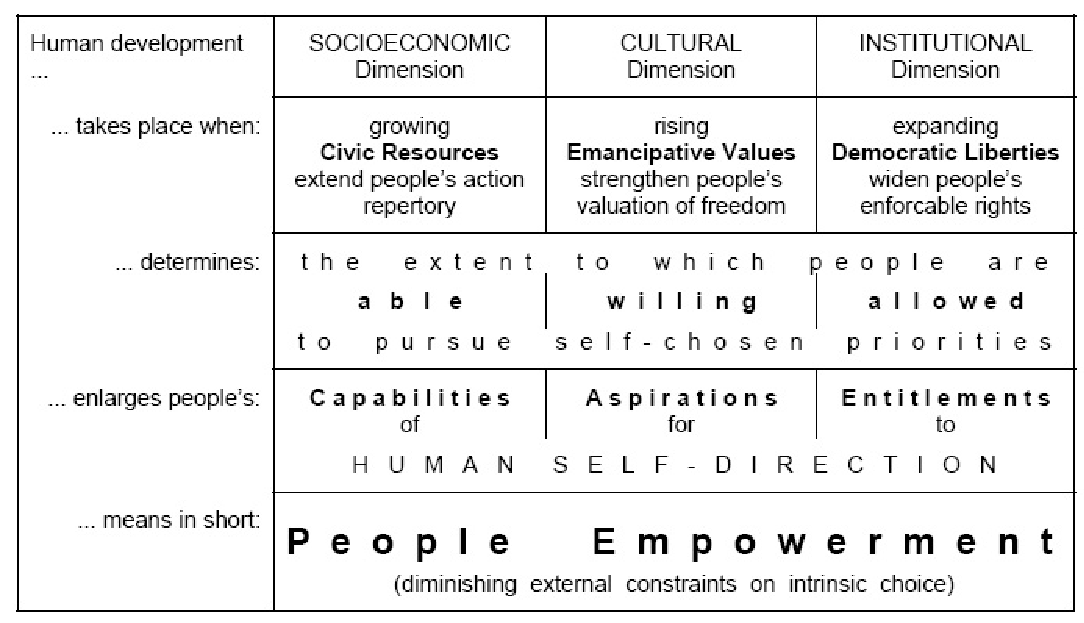
\includegraphics[width=\linewidth]{./SocSci/Welzel-fig002.pdf}
   \mycaption{\normalsize The Human Development of Societies \textit{Source:} Adapted from Welzel (2002:46).} 		  						\label{fig:Welzel002}
   \end{center}
\end{figure} 
\newpage
\begin{figure}[ht]
  \begin{center}
    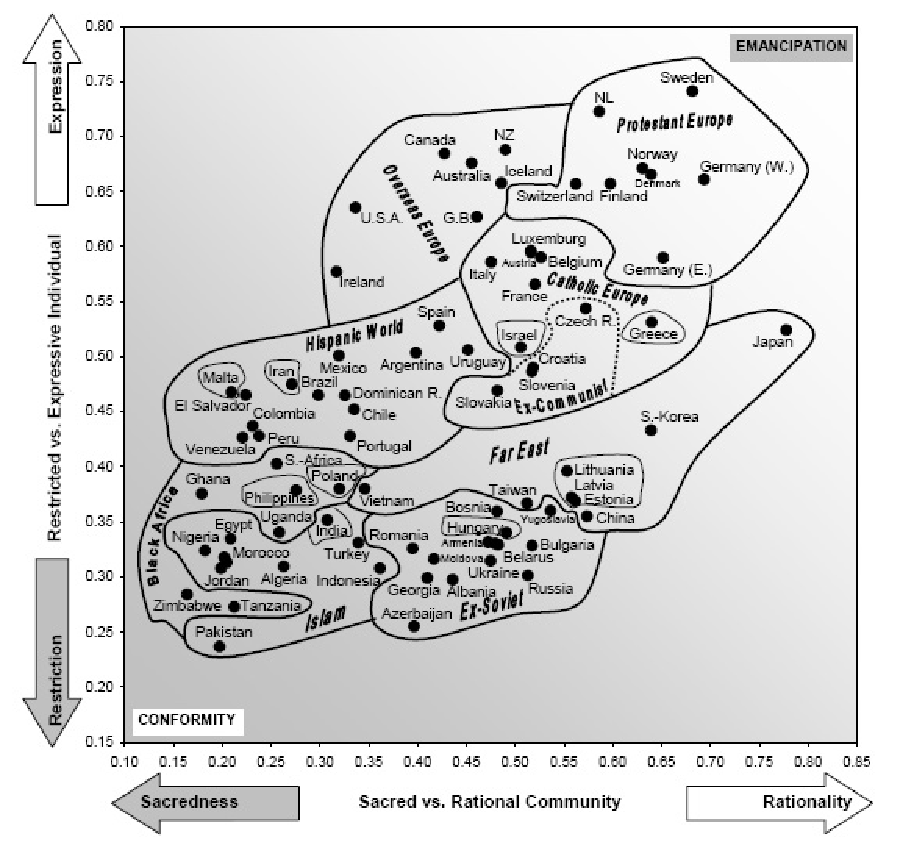
\includegraphics[width=0.9\linewidth]{./SocSci/Welzel-fig001.pdf}
   \mycaption{\normalsize Emancipative Values around the World} \label{fig:Welzel001}
   \end{center}
\end{figure} 


\textbf{Funded Projects}\\[-0.25cm]
\begin{enumerate}
\item[$\bullet$]	World Values Surveys: questionnaire design, coordinating fund raising activities and fieldwork, funded by Bank of Sweden Tercentenary Foundation
\item[$\bullet$]	German part of the World Values Surveys: principal investigator funded by Deutsche Forschungsgemeinschaft
\end{enumerate}


\vspace{0.6cm}
\textbf{Other Professional Activities}\\[-0.25cm]
\begin{enumerate}
\item[$\bullet$]	Member of the scientific advisory board of McKinsey company's "Perspektive Deutschland 2005"
\item[$\bullet$]	Consultant of the GfK's (Gesellschaft f�r Konsumforschung) study on value change
\item[$\bullet$]	Member of an expert group of the EU Commission on value orientations towards science and technology
\item[$\bullet$]	Member of scientific advisory board of the Telekom Foundation's "Innovationsindikator Deutschland"
\item[$\bullet$]	Member of the executive committee of the World Values Surveys Association
\item[$\bullet$]	IUB's official representative to the European Consortium of Political Science (ECPR)
\item[$\bullet$]	Co-organized several meetings of the executive committee of World Values Survey Association at various locations
\end{enumerate}


\newpage
\textbf{PhD-Students}\\[-0.25cm]

Alexander Boloussov\newline
\textit{Determinants of the Density of Human Rights NGOs in Postcommunist Publics}\\[-0.15cm]

Nicola B�cker\newline
\textit{Frames in European Identities in Postcommunist and Non-Postcommunist Publics}\\[-0.15cm]

Franziska Deutsch\newline
\textit{Participation and Democracy - Elite-Challenging Political Action in Old and New Democracies}\\[-0.15cm]

Jan M�ller\newline
\textit{The Influence of Values on the Interpretation of Collective Action Frames}\\[-0.15cm]

Yevgenya Paturyan\newline
\textit{Democratic Potential of Voluntary Associations in Semi-Democratic Postcommunist Regimes}\\[-0.15cm]

Caner Uguz\newline
\textit{Personality Cult in Politics: The Attat�rk Cult in Comparative Perspective}


\vspace{0.6cm}
\textbf{Research Personnel}\\[-0.25cm]

Franziska Deutsch works as research associate in the project "European and World Values Surveys" funded by the Deutsche Forschungsgemeinschaft


